% !TeX program = LuaLaTeX
\documentclass[a4paper,14pt,russian]{extreport}
 
\usepackage{fontspec}
\usepackage[abspath]{currfile}
\setmainfont[
  Path          = \currfileabsdir,
  Ligatures     = TeX,
  UprightFont   = fonts/times.ttf,
  BoldItalicFont= fonts/timesbi.ttf,
  BoldFont      = fonts/timesbd.ttf,
  ItalicFont    = fonts/timesi.ttf
]{Times New Roman}

%\usepackage{extsizes}
\usepackage[russian]{babel}
\usepackage{indentfirst}


\usepackage{amsfonts}
\usepackage{amsmath}
\usepackage{appendix}
\usepackage{comment}

\bibliographystyle{utf8gost705u}

\linespread{1.4} % полуторный интервал
%\renewcommand{\rmdefault}{ftm} % Times New Roman
\frenchspacing

% misc
%\usepackage{fullpage}

\usepackage{hyperref}

% review
\usepackage[textwidth=120]{todonotes}
\usepackage{color}

% graphics
\usepackage{graphicx}

% graphicx configuration
\graphicspath{{image/}}
\DeclareGraphicsExtensions{.pdf,.png,.jpg}
\setcounter{totalnumber}{10}
\setcounter{topnumber}{10}

\usepackage{titlesec} % стиль глав и секций
 
\titleformat{\chapter}[display]
    {\filcenter}
    {\MakeUppercase{\chaptertitlename} \thechapter}
    {8pt}
    {}
 
\titleformat{\section}
    {\normalsize}
    {\thesection}
    {1em}{}
 
\titleformat{\subsection}
    {\normalsize}
    {\thesubsection}
    {1em}{}
    
\newcommand{\empline}{\mbox{}\newline}
\newcommand{\likechapterheading}[1]{ 
    \begin{center}
    \textbf{\MakeUppercase{#1}}
    \end{center}
    \empline}
    
\makeatletter
    \renewcommand{\@dotsep}{2}
    \newcommand{\l@likechapter}[2]{{\bfseries\@dottedtocline{0}{0pt}{0pt}{#1}{#2}}}
\makeatother
\newcommand{\likechapter}[1]{    
    \likechapterheading{#1}    
    \addcontentsline{toc}{likechapter}{\MakeUppercase{#1}}}    

% boarders
\usepackage{geometry}
\geometry{left=2.4cm}
\geometry{right=2cm}
\geometry{top=2cm}
\geometry{bottom=2.5cm}

% fixing numbering problem
\usepackage{chngcntr}
\counterwithout{figure}{chapter}
\counterwithout{table}{chapter}
\counterwithout{equation}{chapter}

\begin{document}

%\documentclass[a4paper]{article}
%\usepackage[14pt]{extsizes} % для того чтобы задать нестандартный 14-ый размер шрифта
%\usepackage[utf8]{inputenc}
%\usepackage[russian]{babel}
%\usepackage{setspace,amsmath}
%\usepackage[left=20mm, top=15mm, right=15mm, bottom=15mm, nohead, footskip=10mm]{geometry} % настройки полей документа
 
%\begin{document} % начало документа
 
% НАЧАЛО ТИТУЛЬНОГО ЛИСТА
\begin{center}
\hfill \break
\small{Министерство образования и науки Российской Федерации}\\
\small{Федеральное государственное автономное образовательное учреждение}\\ 
\small{высшего профессионального образования}\\
\small{\textbf{«Московский физико-технический институт (государственный университет)»}}\\
\hfill \break
\small{Факультет проблем физики и энергетики}\\
\small{Кафедра «Фундаментальные взаимодействия и космология»}\\
\end{center}
%\begin{flushright}
%На правах рукописи \\
%УДК   \underline{\hspace{3cm}} 
%\end{flushright}
\begin{center}
\hfill \break
\normalsize{Полякова Мария Александровна}\\
\large{Практическое применение \\статистической регуляризации Турчина}\\
\hfill \break
\hfill \break
\normalsize{Выпускная квалификационная работа\\
\hfill \break
Направление подготовки:      03.03.01 Прикладные математика и физика}\\
\hfill \break
\end{center}

\hfill \break
\normalsize{ 
\begin{tabular}{cccc}

Научный руководитель & \underline{\hspace{3cm}}& & /А. А. Нозик/ \\\\
Студент & \underline{\hspace{3cm}} & &/М. А. Полякова/ \\\\
\end{tabular}
}\\
\hfill \break
\hfill \break
\hfill \break
\begin{center} Москва \\ 2017 \end{center}
\thispagestyle{empty} % выключаем отображение номера для этой страницы
 
\newpage
%\listoftodos
\tableofcontents
\newpage
\likechapter{Введение}

Наблюдение узких особенностей представляется принципиальной задачей любой (оптической, атомной, ядерной) спектроскопии. В постановке спектрометрических задач экспериментальной физики, как правило, существует противоречие между улучшением разрешаюшей способности прибора для поиска указанных особенностей и интенсивностью сигнала, определяющей статистическую значимость. В тех случаях, когда разрешение улучшить нельзя, и искомая особенность искажена, для ее ``восстановления'' возникает необходимость в решении обратной задачи.
И такие задачи, как правило, некорректны. Это значит, что малые (статистические) флуктуации в измеряемой функции, обуславливают большие флуктуации искомой функции - решения.
В качестве примера некорректно поставленной задачи в работе рассматривается уравнение Фредгольма I рода. Математическая формулировка задачи такова: по известным оператору $\hat{K}$ и функции $f$, найти функцию $\varphi$, являющуюся решением уравнения:
\begin{equation}
\hat{K}\varphi = f.
\label{eq:opereq}
\end{equation}
Данная математическая модель описывает следующую прикладную задачу: восстановить некоторый закон природы (входной сигнал измерительной аппаратуры) по проведенным в эксперименте измерениям (выходному сигналу), при условии, что известна аппаратная функция прибора (оператор, преобразующий входной сигнал в выходной). Поскольку функция $f$ соответствует измеряемым данным, она всегда известна только приближенно. Тогда для некоторых операторов $\hat{K}$, задача окажется некорректной, и малый шум в исходных данных приведет к значительным искажениям в восстановленной функции $\varphi$. 

Разработано достаточно методов решения некорректных обратных задач. Самым распространненым в экспериментальной физике считается метод регуляризации Тихонова \cite{tihonov}. Но существует также иной подход к регуляризации, разработанный Турчиным \cite{turchin}, который основан на Байесовой статистике. Он имеет ряд преимуществ, однако в течении многих лет оставался без внимания ученых. 
\newpage
\likechapter{Литературный обзор}
Статистический метод регуляризации был разработан Турчиным и описан в статье \cite{turchin}. В диссертации \cite{turovceva} рассматривается применение этого метода для решения некоторых задач атмосферной физики. Данные две работы послужили основой теории настоящей выпускной квалификационной работы.


Методы с использованием Байесовой статистики для регуляризации рассмотрены в статьях \cite{review1}, \cite{rev1995}, \cite{rev:emper}, однако без рассмотрения дополнительных возможностей, таких как определение погрешности найденного решения и добавления дополнительной априорной информации. В статье \cite{rev2009} обсуждается решение проблемы выбора наилучшего значения параметра регуляризации с использованием метода максимального правдоподобия. Также ранее уже рассматривалось использование Байесовой статистики для восстановления изображений \cite{rev1972}, обработки данных позитронно-эмиссионной томографии \cite{rev1985a} и однофотонной эмиссионной компьютерной томографии \cite{rev1985b}.
\newpage
\chapter{ОПИСАНИЕ МЕТОДА}

Метод регуляризации подробно изложен в статье \cite{turchin}. Текст оригинальной работы достаточно сложно найти, поэтому мы изложим в этом обзоре основные положения методики

\section{Стратегия}
Статистический метод регуляризации основан на Байессовой статистике и методе принятии решений в условии неопределенности. Сначала необходимо перейти из непрерывного пространства функций в параметризованное дискретное представление. Такой переход называется алгебраизацией. В результате функции $f$ и $\varphi$ превращаются в вектора, а оператор $\hat{K}$ в матрицу. В результате уравнение (\ref{eq:opereq}) преобразуется в
\begin{equation}
  f_m = K_{mn}\varphi_n,
\label{eq:algebr}
\end{equation}
где $f_m$ --- набор (вектор) случайных величин с известной плотностью вероятности, представляющих собой результат измерения в конечном числе $M$ точек $y_m$ на отрезке $[c;d]$; $\varphi_n$ --- вектор, задающий алгебраизацию исследуемого закона природы (функции $\varphi$), $K_{mn}$ --- известная матрица, задающая преобразование $\vec{\varphi}$ в  $\vec{f}$.
В результате исходную задачу можно переформулировать следующим образом: по известной реализации $\vec{f}$ нам нужно оценить значение параметра $\vec{\varphi}$. Функцию $\vec{S}$, которая определяется как алгоритм нахождения оценок $\vec{\varphi}$ на основе $\vec{f}$, мы будем называть стратегией. 

В общем случае форма произвольной функции описывается бесконечномерным вектором, поэтому описание при помощи вектора конечной размерности приводит к частичной потере информации. Методика никак не ограничивает набор базисных функций, по которым производится разложение, но выбор конкретных параметров алгебраизации существенно влияет на результат работы. Примеры различных способов алгебраизации будут рассмотрены в ниже.

Для сравнения результатов, полученных с помощью разных стратегий, вводится \textit{квадратичная функция потерь}:

\begin{equation}
	L(\hat{\vec{\varphi}},\vec{S}) = \sum\mu_n(\hat{\varphi}_n-S_n)^2,
\end{equation}
где $\hat{\vec{\varphi}}$ --- наилучшее решение, а $\mu_n$ --- весовой коэффициент. Тогда для некоторого решения $\varphi$ потери выбранной нами стратегии задаются \textit{функцией риска}:

\begin{equation}
	R_{\vec{S}}(\vec{\varphi}) \equiv E[L(\vec{\varphi},\vec{S})] = \int L(\vec{\varphi},\vec{S})P(\vec{f}|\vec{\varphi})d\vec{f}, 
\end{equation}
где $P(\vec{f}|\vec{\varphi})$ --- это плотность вероятности ансамбля, по которому производится усреднение потерь. Этот ансамбль образован гипотетическим многократным повторением  измерений $\vec{f}$ при заданном $\vec{\varphi}$, таким образом $P(\vec{f}|\vec{\varphi})$ это та самая известная нам плотность вероятности $\vec{f}$, полученная в эксперименте.

Согласно Байессовскому подходу предлагается рассмотреть $\vec{\varphi}$, как \textbf{случайную переменную} с \textit{априорной плотностью вероятности} $P(\vec{\varphi})$, выражающую \textbf{достоверность} различных возможных законов природы. $P(\vec{\varphi})$ определяется на основе информации, существующей до проведения эксперимента \cite{chernov}. Тогда выбор оптимальной стратегии основывается на минимизации \textit{апостериорного риска}:
\begin{equation}
	r_{\vec{S}}(\vec{\varphi}) \equiv E_{\vec{\varphi}}E_{\vec{f}}[L(\vec{\varphi},\vec{S})|\vec{\varphi}].
\end{equation}
В этом случае оптимальная стратегия хорошо известна:
\begin{equation}
	\label{eq:opt}
	\vec{S}_{opt} = E[\vec{\varphi}|\vec{f}] =\int \varphi_n P(\vec{\varphi}|\vec{f})d\vec{\varphi},
\end{equation}

\noindent  где \textit{апостерионая плотность} $P(\vec{\varphi}|\vec{f})$ определяется по теореме Баейса:

\begin{equation}
P(\vec{\varphi}|\vec{f})= \frac{P(\vec{\varphi})P(\vec{f}|\vec{\varphi})}{\int d\vec{\varphi}P(\vec{\varphi})P(\vec{f}|\vec{\varphi})} .
\end{equation}

\noindent Кроме того, такой подход позволит определить дисперсию полученного решения:

\begin{equation}
\left\langle \sigma_n^2 \right\rangle = \int (\varphi_n - S^{opt}_n)^2 P(\vec{\varphi}|\vec{f})d\vec{\varphi}.
\end{equation}

Итак, мы получили оптимальное решение уравнения (\ref{eq:opereq}), введя априорную плотность $P(\vec{\varphi})$. Метод статистической регуляризации основан на введении априорной информации о $\varphi(x)$. Если исследователь уже обладает какой-либо априорной информацией (априорной плотностью $P(\vec{\varphi})$, он может просто посчитать интегралы (\ref{eq:opt}) и получить ответ. Для случая, если такой информации нет, в следующем параграфе описывается, какой минимальной информацией может обладать исследователь и как её использовать для получения регуляризованного решения.

\section{Априорная информация}

При работе с Байесовской статистикой ключевым вопросом всегда является выбор априорной вероятности, специфичной для конкретной задачи. Наиболее часто встречающееся в физике ограничение на вид исследуемых функций - это требование непрерывности и гладкости, причем под гладкостью подразумевается не только наличие непрерывной второй производной, но и ее сравнительно маленькое значение. Это связано с тем, что в физических процессах как правило не бывает резких перепадов. Требование минимальной гладкости является очевидным выбором для априорной информации. Поскольку конкретное ограничение на значение второй производной обычно неизвестно, можно также потребовать, чтобы дополнительная информация, возникающая в результате ограничения была минимальной.

Эту задачу можно формализовать следующим образом: требуется найти $P(\vec{\varphi})$, при котором функционал информации Шеннона:

\begin{equation}
	\label{eq:inforamation}
	I[P(\vec{\varphi})] = \int \ln{P(\vec{\varphi})} P(\vec{\varphi}) d\vec{\varphi}
\end{equation}
минимален, и при этом выполнялись следующие условия:
\begin{enumerate}
	\item Плотность вероятности нормированна на единицу:
	\begin{equation}
		\int P(\vec{\varphi}) d\vec{\varphi} = 1
	\end{equation}
	
	\item Условие на гладкость $\varphi(x)$. Пусть $\Omega$ --- некоторая матрица характеризующая гладкость функции. Тогда потребуем, чтобы достигалось определённое значение функционала гладкости:
	\begin{equation}
		\label{eq:glad}
		\int (\vec{\varphi},\Omega\vec{\varphi}) P(\vec{\varphi}) d\vec{\varphi} = \omega,
	\end{equation}
	Обратим внимание на два обстоятельства. Во-первых, значение параметра $\omega$, скорее всего, неизвестно, и способы его определения будут рассмотрены далее в обзоре. Во-вторых, мы уже неявно использовали априорную информацию о гладкости функции, когда определяли функцию полезности: квадратичная функция полезности является хорошим выбором, потому что любая регулярная функция, вблизи экстремума хорошо приближается квадратичной формой.
\end{enumerate}

Эта задача решена в \cite{turchin}, решение приведено в приложении \ref{sec:metod}. В результате преобразований получается следующее решение:

\begin{equation}
	\label{eq:apriori}
	P_{\alpha}(\vec{\varphi})  = \frac{\alpha^{Rg(\Omega)/2}\det\Omega^{1/2}}{(2\pi)^{N/2}} \exp(-\frac{1}{2} (\vec{\varphi},\alpha\Omega\vec{\varphi})),
\end{equation}
где $\alpha = 1/\omega$. 
Значение параметра $\alpha$ на этом этапе неизвестно, и может быть получено следующими способами:

\begin{itemize}
	\item напрямую из каких-то внешних данных или подобрано вручную (в этом частном случае результаты работы метода эквиваленты регуляризации Тихонова \cite{tihonov},
	\item как максимум апостериорной информации $P(\alpha|\vec{f})$,
	\item как среднее по всем возможным $\alpha$, определив априорную плотность вероятности как:
		\begin{equation}
			P(\vec{\varphi}) = \int d\alpha P(\alpha) P(\vec{\varphi}|\alpha),
		\end{equation}
		причем в соответствии с байесовским подходом, можно принять все $\alpha$ равновероятными.
\end{itemize}

\section{Случай гауссовых шумов}

Наиболее распространенным в экспериментальной физике является случай, когда разброс результатов эксперимента подчиняется нормальному распределению. В этом случае регуляризация имеет аналитическое решение.
Пусть вектор измерений $f$ имеет ошибки, описываемые многомерным гауссовым распределением с ковариационной матрицей $\Sigma$:

\begin{equation}
	P(\vec{f}|\vec{\varphi}) = \frac{1}{(2\pi)^{M/2}|\Sigma|^{1/2}} \exp(-\frac{1}{2}(\vec{f} - K\vec{\varphi})^T\Sigma^{-1}(\vec{f} - K\vec{\varphi}))
	\label{eq:gaussP}
\end{equation}

Будем искать оценку $\alpha$, как наиболее вероятное по апостериорной плотности вероятности $P(\alpha|\vec{f})$. В \cite{turchin} показано, что для этого нужно взять $\alpha*$, при котором достигается максимум функции: 

\begin{equation}
	\label{eq:alphamax}
	F(\alpha,\vec{f}) = \frac{Rg(\Omega)}{2}\ln{\alpha} - \frac{1}{2}\ln{|B+\alpha\Omega|}  + \frac{1}{2}b^{T}(B+\alpha\Omega)^{-1}b
\end{equation}
Такой максимум должен существовать, к тому же, при наличии достоточной информации для существования разумного решения, дисперсия $P(\alpha|f)$ не должна быть слишком большая. Тогда подставив найденное значение наиболее вероятного $\alpha^*$ в выражение для апостериорной вероятности $\vec{\varphi}$:  
\begin{comment}Вообще говоря, наша выборка $\vec{f}$ не обязана содержать достаточно информации для существования наиболее вероятного $\alpha^*$. При обработке данных следует проверить этот факт, исследовав функцию \begin{equation}
	\label{eq:alphaaposter}
	P(\alpha|\vec{f}) = C \alpha^{\frac{Rg(\Omega)}{2}}\sqrt{|(B+\alpha\Omega)^{-1}|}\exp(-\frac{1}{2}b^{T}B^{-1}b)\exp(\frac{1}{2}b^{T}(B+\alpha\Omega)^{-1}b)
\end{equation}
Если же наше предположение оправдано, то подставим полученное $\alpha^*$ в выражение для апостериорной вероятности $\vec{\varphi}$:
\end{comment}

\begin{gather*}
	P(\vec{\varphi}|\vec{f})= \frac{P(\vec{\varphi})P(\vec{f}|\vec{\varphi})}{\int d\vec{\varphi}P(\vec{\varphi})P(\vec{f}|\vec{\varphi})} = \\
	=\frac{1}{(2\pi)^{N/2}|(K^T\Sigma^{-1}K+\alpha^*\Omega)^{-1}|^{1/2}} \times \\
	\times \exp(-\frac{1}{2} (\vec{\varphi},(K^T\Sigma^{-1}K + \alpha^*\Omega)\vec{\varphi}) + K^T\Sigma^{-1T}\vec{f}\vec{\varphi})
\end{gather*}
Поскольку апостериорная плотность вероятности получилась гауссовой, а наилучшее решение является математическим ожидание данного распределения, не составляет труда выписать это решение и его ковариационную матрицу (по которой можно определить ошибки, согласно приложению ~\ref{sec:gauss}):

\begin{equation} \label{eq:analit_solv}
	\vec{S}_{opt} = (K^T\Sigma^{-1}K+\alpha^*\Omega)^{-1}K^T\Sigma^{-1T}\vec{f}
\end{equation}

\begin{equation}
	\texttt{cov}(\varphi_m, \varphi_n) = ||(K^T\Sigma^{-1}K+\alpha^*\Omega)^{-1}||_{mn}
\end{equation}

\chapter{ПРИМЕНЕНИЕ РЕГУЛЯРИЗАЦИИ НА ПРАКТИКЕ}

Описанная в \cite{turchin} и предыдущем разделе методика дает теоретический базис для решения многих задач анализа данных. Для практического применения необходимо также исследовать поведение результатов в зависимости от типа восстанавливаемой функции, а также от параметров алгебраизации и др. Сравнение работы метода при использовании различных базисов было проверено на нескольких модельных задачах. Для исследования работы метода заданная функция $\varphi$ свертывалась с интегральным ядром $K$, и к полученным значениям добавлялась случайная погрешность, имеющую нормальное распределение со средним равным нулю и шириной в 1\% от максимального значения функции на отрезке. Полученные данные обрабатывались описанным выше методом, реализующим аналитическое решение (\ref{eq:analit_solv}).


\section{Выбор параметра регуляризации}

При использовании статистического метода регуляризации удается последовательно получить распределение $P(\alpha | f)$, и вместо использования одного выбранного значение параметра регуляризации, можно произвести усреднение по всем возможным значениям параметра. Усреднение (интегрирование) производилось методом Монте-Карло с использованием метода существенной выборки. Однако, при достаточно узком распределении апостериорной вероятности $P(\alpha)$ интегрирование можно заменить нахождением наиболее вероятного $\alpha$, нахождением экстремума функции (\ref{eq:alphaaposter}) (Приложение \ref{sec:metod}). На Рис.\ref{pic:13} можно видеть, что оба метода дают схожий результат, однако при интегрировании уменьшаются погрешности найденного решения.

\begin{figure}[h! ]
	\label{pic:13}
	\center{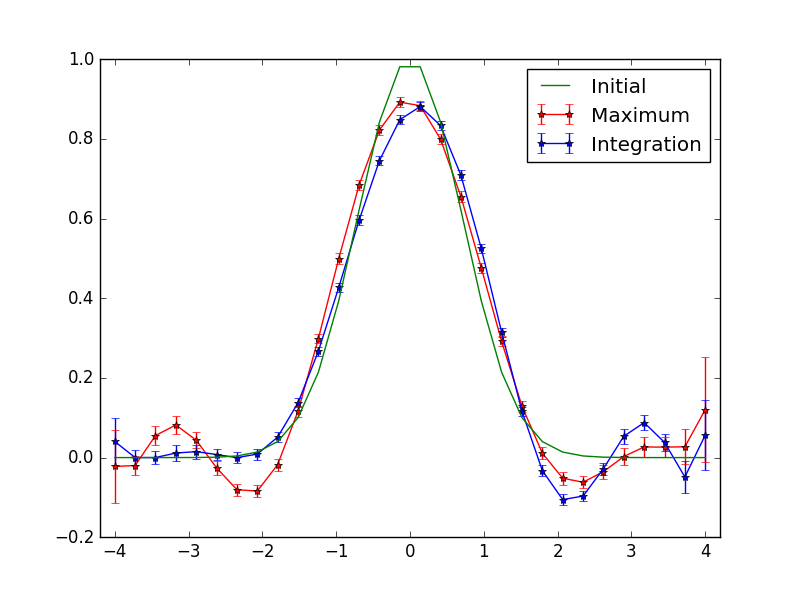
\includegraphics[scale=0.45]{integrate}}
	\caption{Результат восстановления функции с использованием усреднения по $\alpha$ (синяя кривая) и с поиском наиболее вероятного $\alpha$ (красная кривая).}
\end{figure}

\section{Базис алгебраизации}

Как было указано выше, метод регуляризации не ограничивает выбор конкретного базиса для разложения функций. В этом разделе будет представлено исследование зависимости результата регуляризации от выбора базиса. Описание математической процедуры алгебраизации уравнения (\ref{eq:opereq}) для разных базисов приведено в Приложении \ref{algebra}.

Ранее, в работе \cite{turovceva}, метод статистической регуляризации был реализован с использованием простейшего способа алгебраизации, в котором в качестве элементов $f_n$ использовались измеренные экспериментальные значения. В данной работе использовались три вида базисов: ряды Фурье, полиномы Лежандра и В-сплайны (описание базисов приведено в Приложениях \ref{sec:fourier}, \ref{sec:legendre} и \ref{sec:spline} соответственно). Сравнение работы метода при использовании различных базисов было проверено на нескольких модельных задачах.

Проведем сравнение восстановления функции с использованием разных базисов в условиях погрешностей эксперимента порядка 1\%. Для этого создадим для базисов равные условия --- одинаковую длину вектора $\phi$. Влияние величины погрешности на результат регуляризации будет рассмотрено в разделе ниже.

На рис.\ref{pic:gauss_3basis} представлено восстановление функции $\varphi(x)=e^{-x^2/2}$. Как можно увидеть из рис.\ref{pic:gauss_3basis}, метод успешно восстанавливает искомую функцию при использовании всех трех исследуемых базисов с незначительными различиями в результатах. 

На рис.\ref{pic:sigmoida_3basis} представлено восстановление сигмоиды $\varphi(x) = \frac{1}{1+e^{-x}}$. На примере этой функции становится заметна особенность базиса Фурье, а именно восприимчивость к асимптотике. При использовании базиса Фурье решение ``стремится'' быть симметричным на концах отрезка, что дает неправильное описание в случае асимметричной асимптотики. Это накладывает некоторые ограничения на использование того или иного базиса для исследования конкретной задачи.

\newpage
 \setlength{\textfloatsep}{10pt plus 1.0pt minus 2.0pt}
\setlength{\floatsep}{5pt plus 1.0pt minus 1.0pt}
\setlength{\intextsep}{5pt plus 1.0pt minus 1.0pt}

\begin{figure}[htbp! ]
	\center{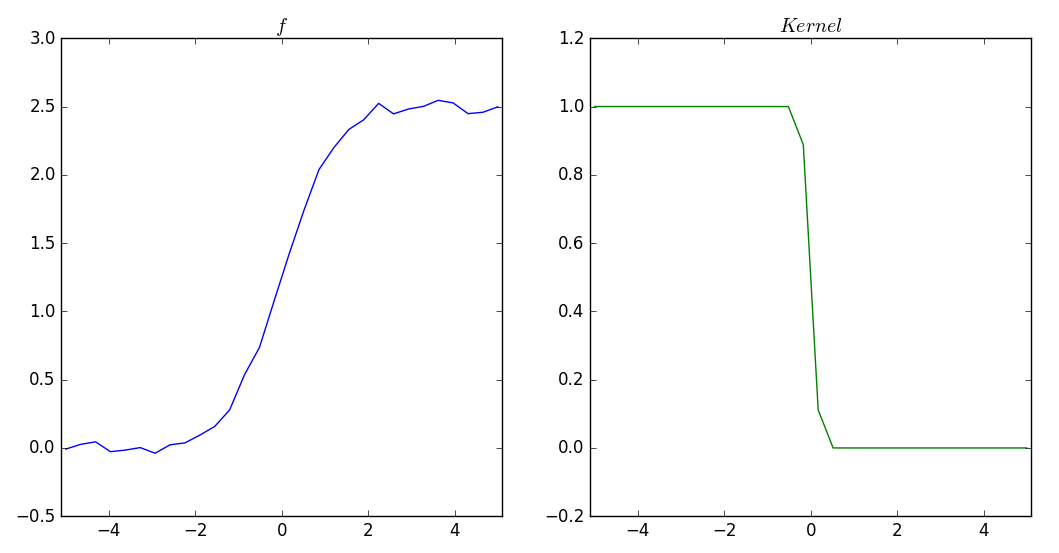
\includegraphics[width=0.7\linewidth]{new_figure_4} \\а)}
	\center{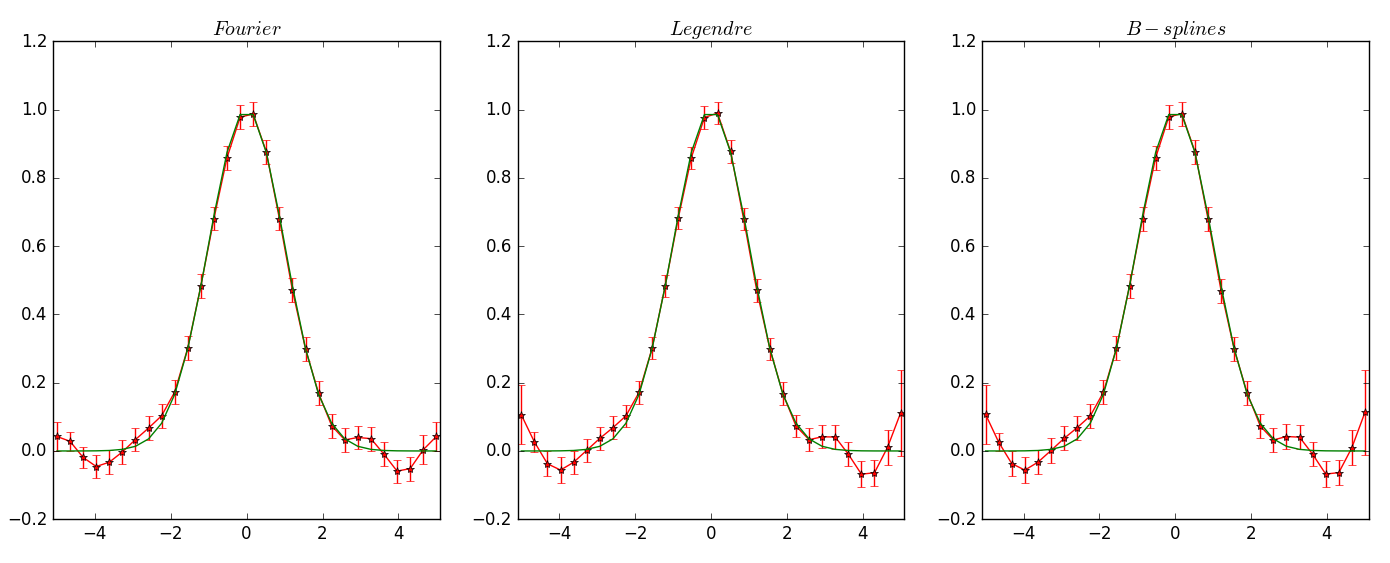
\includegraphics[width=1\linewidth]{new_figure_1} \\б)}
	\caption{Восстановление функции $e^{-x^2/2}$ со статистической погрешностью 1\%, 30 компонент, 30 узлов. Зеленая линия --- исходная функция, красная линия с точками --- результат регуляризации.}
	\label{pic:gauss_3basis}
\end{figure}

\begin{figure}[htbp! ]
	\center{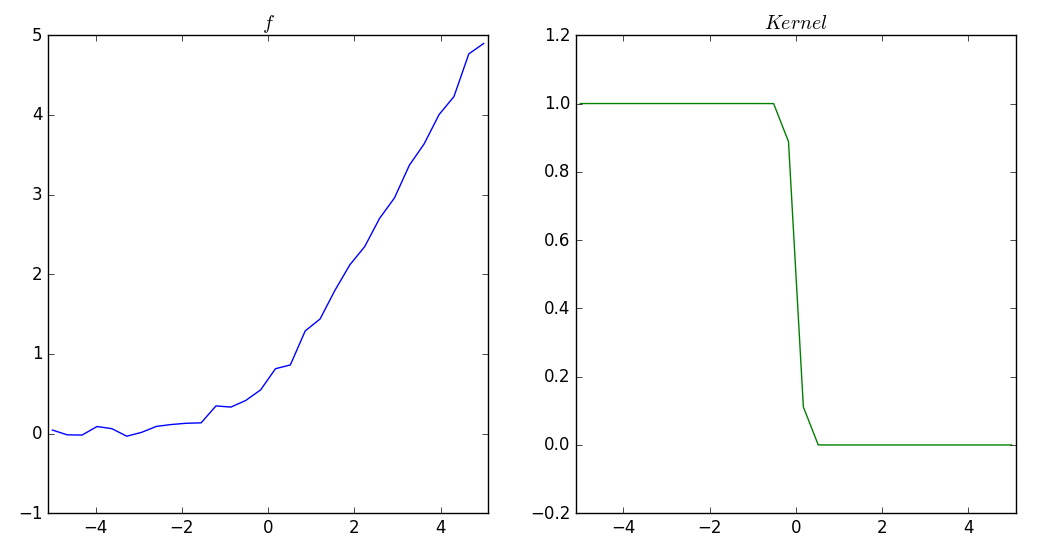
\includegraphics[width=0.8\linewidth]{new_figure_3} \put(0,0){a)}   }
	\center{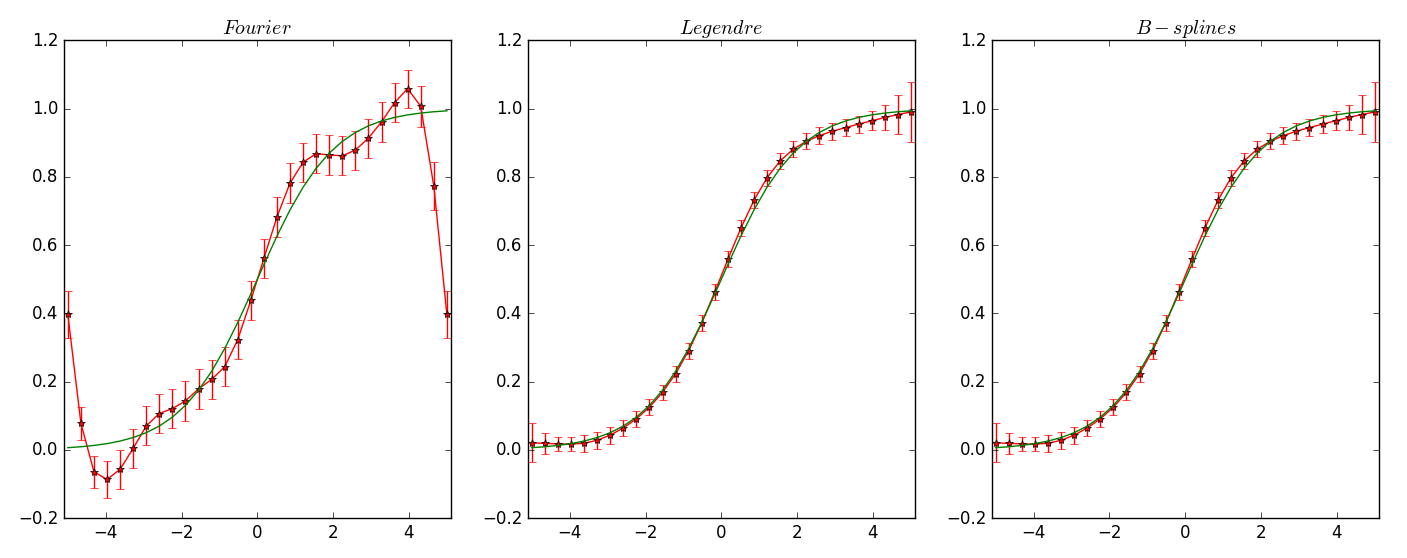
\includegraphics[width=1\linewidth]{new_figure_2} \\б)}
	\caption{Восстановление «сигмоиды» в трех базисах, малые погрешности (1\%) , 30 компонент, 30 узлов. Зеленая линия --- исходная функция, красная линия с точками --- результат регуляризации.}
	\label{pic:sigmoida_3basis}
\end{figure}
\newpage

\subsection{Количество базисных функций}

При задании базиса из полиномов Лежандра или компонент Фурье необходимо выбрать определенное число базисных функций. Рассмотрим влияние выбора этого числа для каждого из базисов. На Рис.\ref{pic:6} и Рис.\ref{pic:7} представлено восстановление функции Гаусса с помощью разного числа компонент в базисах полиномов Лежандра и рядов Фурье соответственно.

\begin{comment}
\begin{figure}[h! ]
	\label{pic:6}
	\center{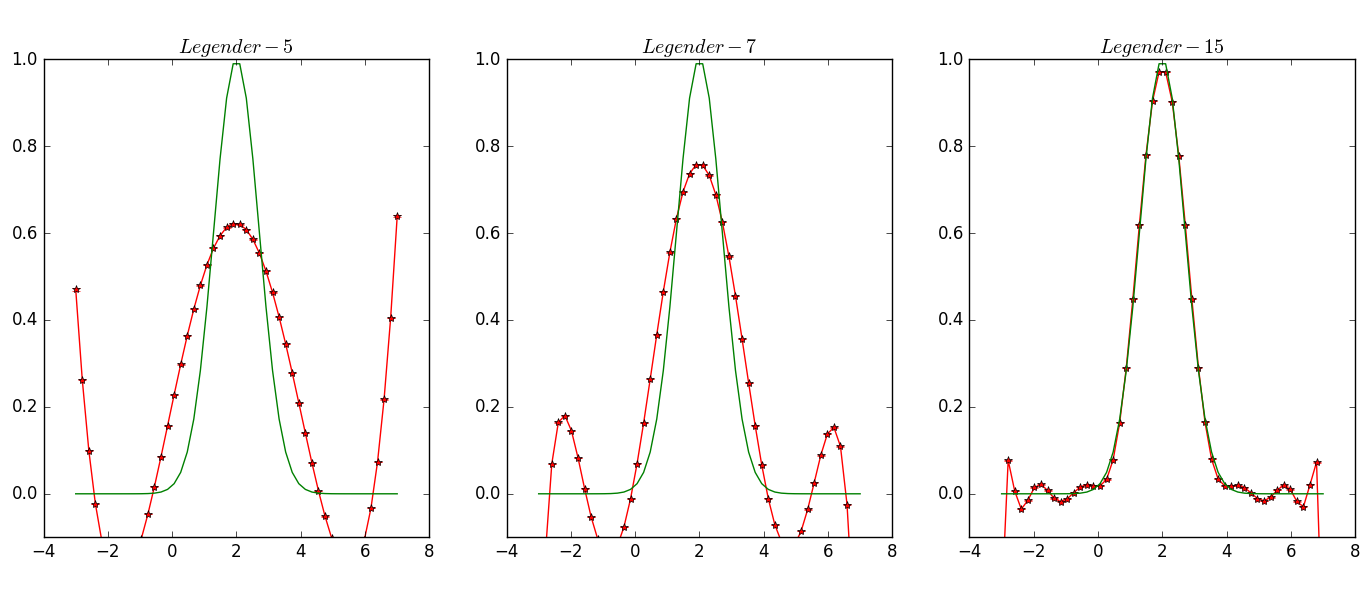
\includegraphics[width=1\linewidth]{pic6} }
	\caption{Восстановление функции Гаусса $e^{-(x-2)^2}$ с помощью 5, 7 и 15 полиномов Лежандра соответственно. Зеленая линия --- исходная функция, красная линия с точками --- результат восстановления.}
\end{figure}


\begin{figure}[h! ]
	\label{pic:7}
	\center{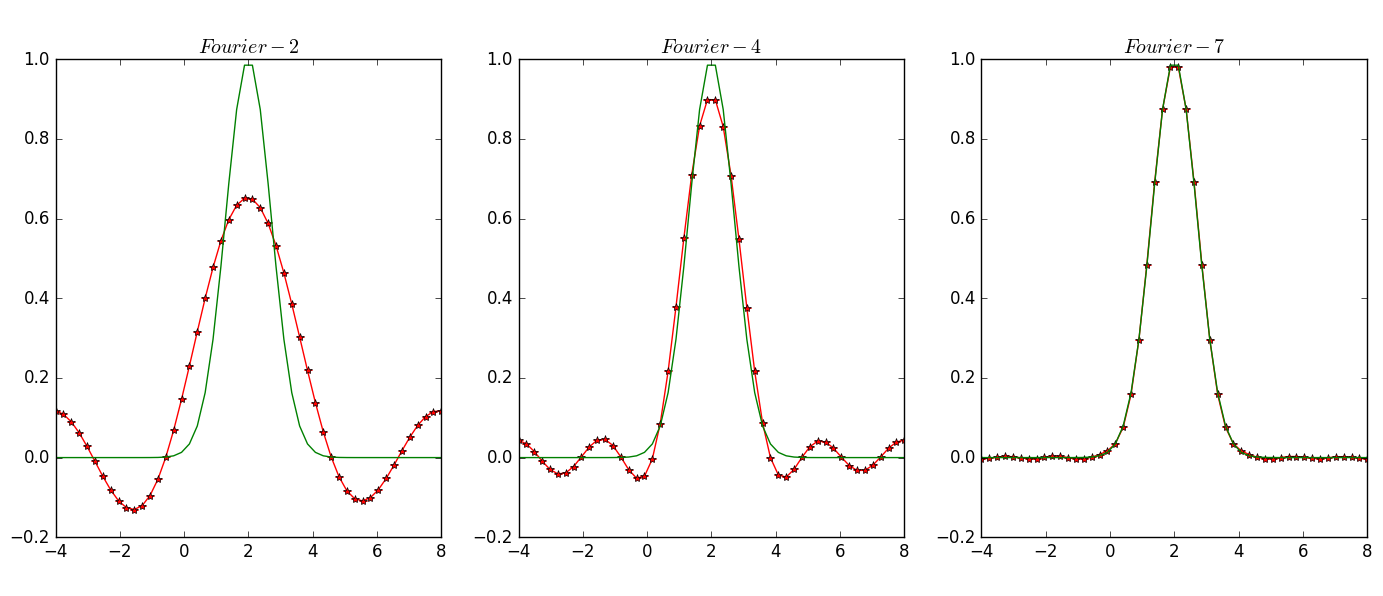
\includegraphics[width=1\linewidth]{pic7}}
	\caption{Восстановление функции Гаусса $e^{-(x-2)^2}$ с помощью 4, 8 и 14 компонент Фурье соответственно. Зеленая линия --- исходная функция, красная линия с точками --- результат восстановления.}
\end{figure}
\end{comment}

Как можно видеть, при использовании базиса полиномов Лежандра необходимо большее число компонент для получения хорошего описания, чем при использовании базиса Фурье. Следовательно при использовании полиномов Лежандра требуется больше вычислительного времени, что является особенностью данного базиса. На Рис.\ref{pic:graf1} представлены графики зависимостей среднего квадрата отклонения от исходной функции и средней погрешности решения от числа базисных компонент. Как видно из данных графиков, значение отклонения и погрешностей с ростом числа компонент выходит на константу, значит можно выбрать оптимальное число базисных компонент для восстановления, дальнейшее добавление базисных функций не будет значительно улучшать результат восстановления.
В целом, говоря о необходимом количестве базисных компонент, стоит заметить, что в методе происходит восстановление именно разложенной по базису функции. Следовательно, значительное влияние на результат имеет именно качество алгебраизации уравнения Фредгольма. 
\begin{comment}
\begin{figure}[h! ]
	\label{pic:7}
	\center{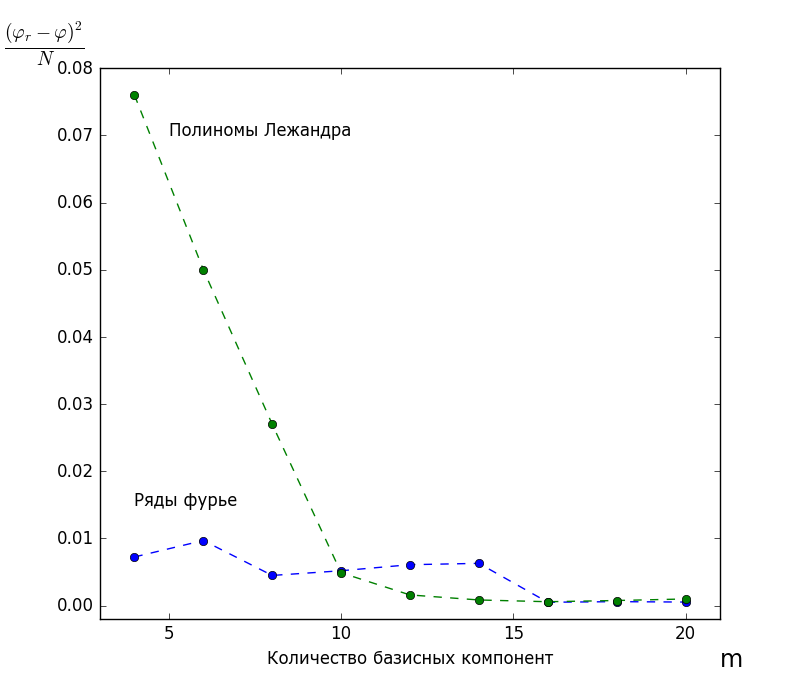
\includegraphics[width=0.9\linewidth]{legendre_and_fourier_components}}
	\caption{График для разных значений m для лежандров и фурье.}
\end{figure}
\end{comment}

\begin{figure}[h! ]
\begin{center}
\begin{minipage}[h]{0.48\linewidth}
	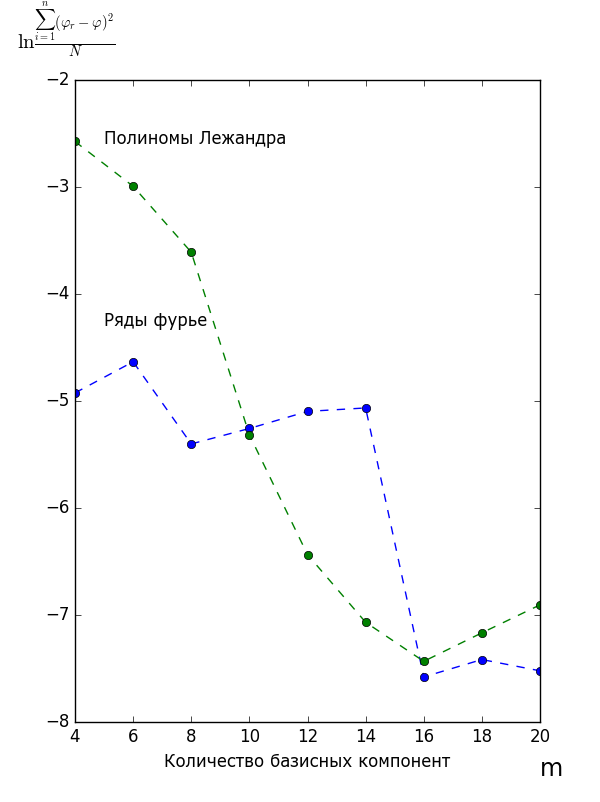
\includegraphics[width=0.9\linewidth]{log_legendre_and_fourier_components} \\а)
\end{minipage}
	\hfill
\begin{minipage}[h]{0.48\linewidth}
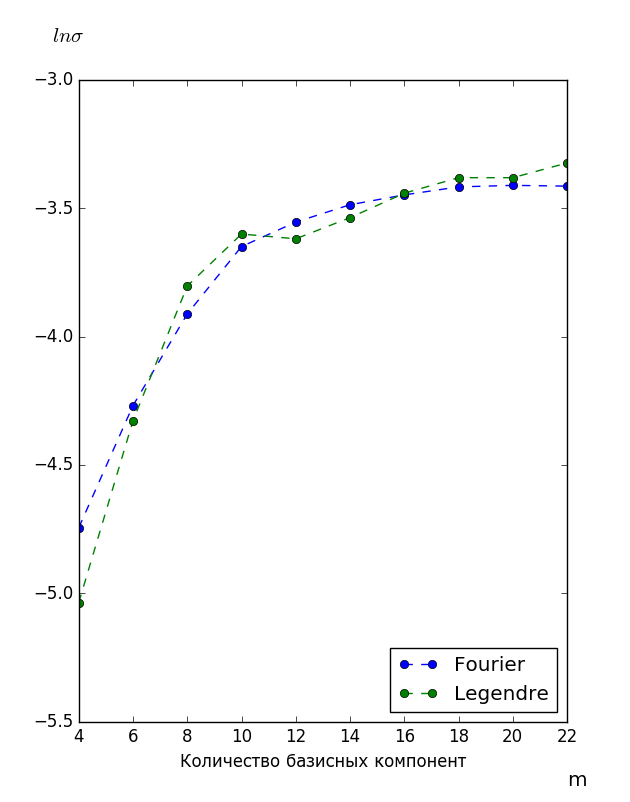
\includegraphics[width=0.9\linewidth]{log_sigma} \\б)
\end{minipage}
	\caption{а) Зависимость среднего квадрата отклонения от количества базисных компонент. б) Зависимость средней погрешности решения от количества базисных компонент}
\label{pic:graf1}
\end{center}
\end{figure}


\subsection{Количество экспериментальных точек и узлов сетки}

Изучим теперь свойства базиса B-сплайнов, зависящих от количества экспериментальных точек (узлов). Аналогично ситуации с числом базисных компонент, при увеличении числа узлов на отрезке средний квадрат отклонения от исходной функции выходит на константу (Рис.\ref{pic:graf2})
\begin{figure}[h! ]
	\label{pic:7}
	\center{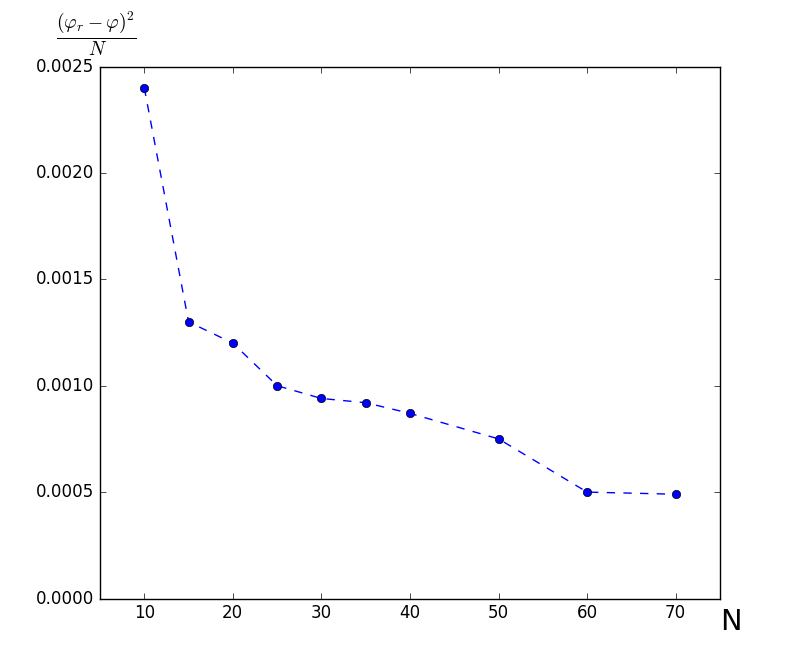
\includegraphics[width=0.75\linewidth]{splines_knots}}
	\caption{График зависимости среднего квадрата отклонения от числа узлов для В-сплайнов.}
	\label{pic:graf2}
\end{figure}


\section{Ядро}

Все случаи, рассмотренные выше, относились к восстановлению функций, свернутых с интегральным ядром. Теперь рассмотрим случай Гауссовского ядра $K=e^{-(x-2)^2}$ (Рис.\ref{pic:gausskernel}) Результат свертки данного ядра с исходной функцией Гаусса показан на Рис.\ref{pic:gausskernel}. Как можно увидеть, в случае неинтегрального ядра исходная функция также успешно восстановлена. Однако, как и в случае рассмотрения разных базисов, нельзя утверждать, что метод и выбранный базис универсален для всех типов ядер.

\begin{comment}
\begin{figure}[h! ]
\begin{center}
\begin{minipage}[h]{0.3\linewidth}
	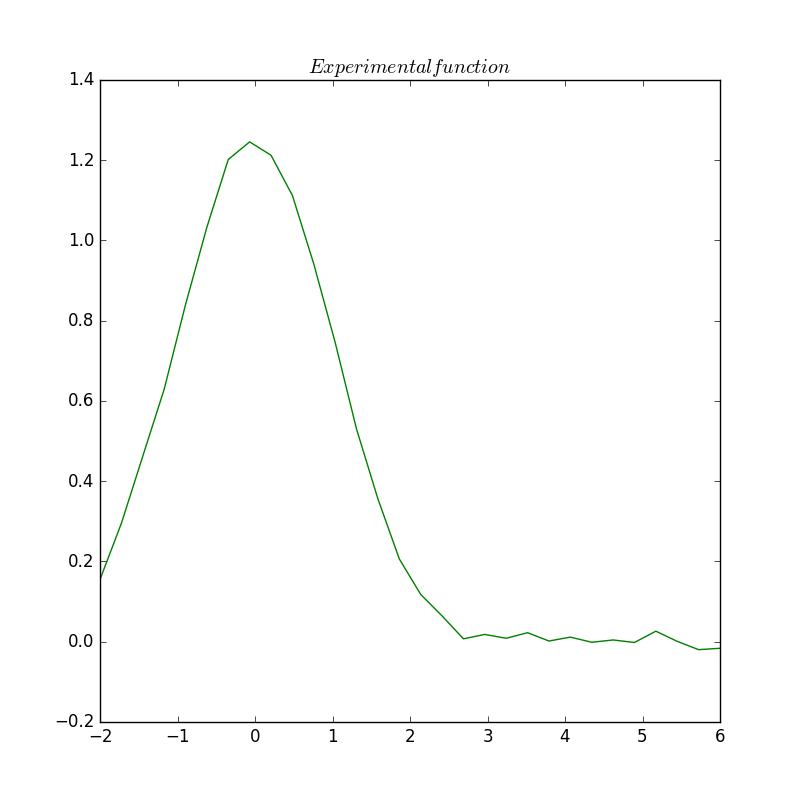
\includegraphics[width=1\linewidth]{func_10} \\а)
\end{minipage}
	\hfill
\begin{minipage}[h]{0.3\linewidth}
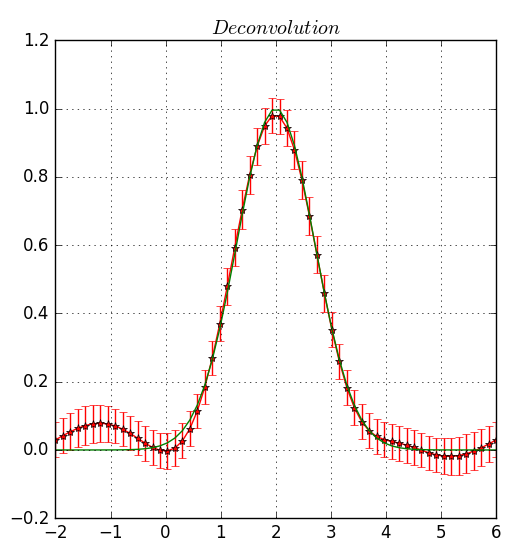
\includegraphics[width=1\linewidth]{pic10a} \\б)
\end{minipage}
\hfill
\begin{minipage}[h]{0.3\linewidth}
	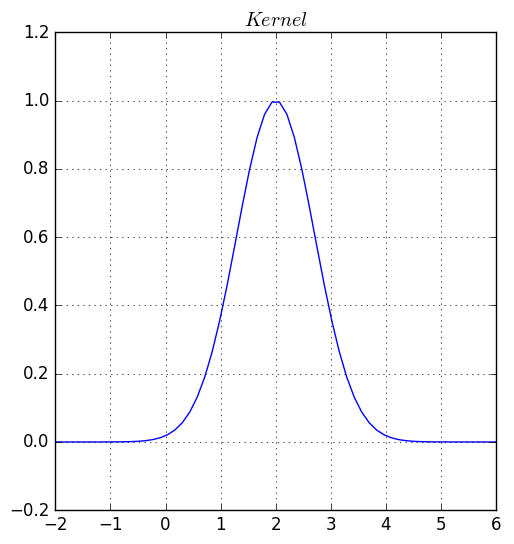
\includegraphics[width=1\linewidth]{pic10b} \\в)
\end{minipage}
	\caption{Случай неинтегрального ядра. а) Экспериментальные значения. б) Ядро $K=e^{-(x-2)^2}$. в) Результат восстановления с помощью базиса Фурье (20 компонент) со статистическими погрешностями 1\%, зеленая линия --- исходная функция, красная линия с точками --- результат регуляризации.}
\label{pic:gausskernel}
\end{center}
\end{figure}
\end{comment}
   
\section{Влияние погрешностей измерения}

Проанализируем влияние величины шумов при измерении на восстановление функции. Для определенности все операции будем проводить в базисе Фурье. На Рис.\ref{pic:noize}. представлено восстановление функции Гаусса в случае разных случайных погрешностей вплоть до 10\%. При восстановлении использовался базис Фурье.

Для успешной работы метода недопустимы нулевые случайные погрешности, так как это приведет к сингулярности при обращении матрицы $\Sigma$ (см. формулу (\ref{eq:gaussP})). Поэтому для моделирования случая с нулевыми шумами были использованы достаточно малые погрешности - 0.001\%. Восстановление в случае с нулевыми ошибками просто соответствует решению интегрального уравнения и восстановленное решение должно совпадать с исходной функцией.

Как можно видеть из Рис.\ref{pic:noize}, при малых статистических ошибках восстановленная кривая совпадает с исходной функцией, что полностью согласуется с ожиданием. Погрешности восстановления также очень малы.

\begin{comment}
\begin{figure}[h! ]
	\center{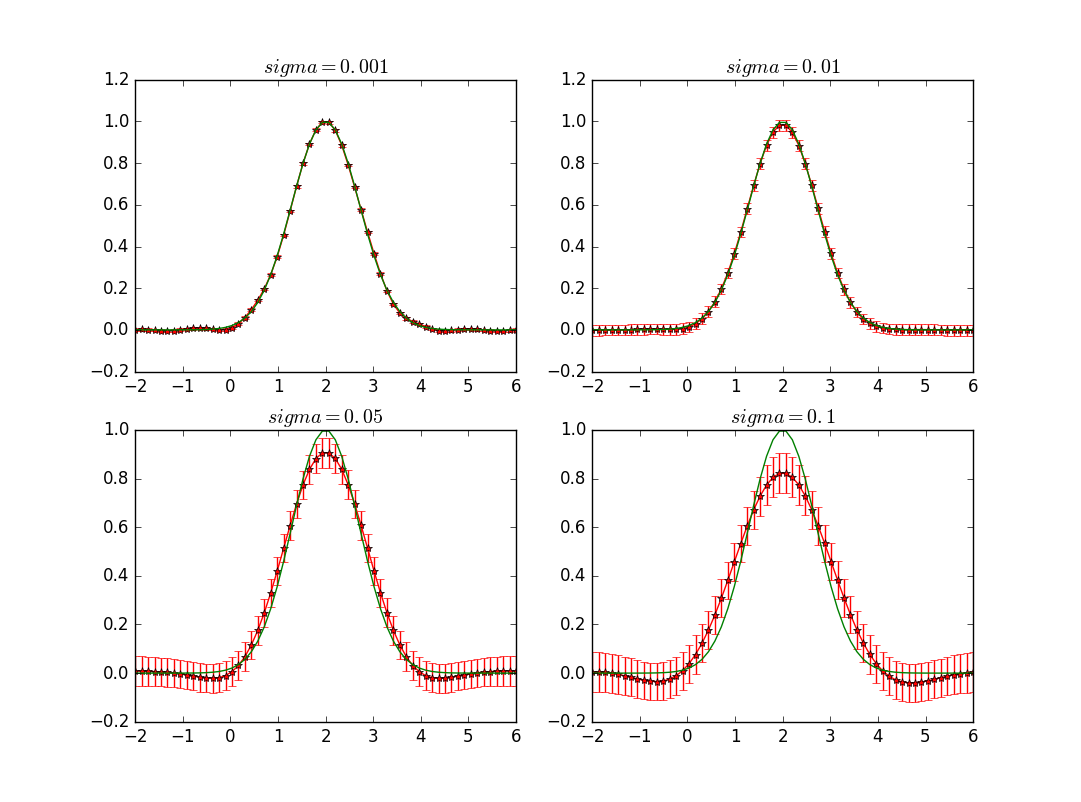
\includegraphics[scale=0.45]{pic12}}
	\caption{Восстановление гаусса с разными погрешностями при измерении: 0.001\%, 1\%, 5\% и 10\%. Зеленая линия --- исходная функция, красная линия с точками --- результат восстановления.}
	\label{pic:noize}
\end{figure}
\end{comment}

Увеличение случайных погрешностей при измерениях искажает решение, делая пик более сглаженным, а также приводит к увеличению погрешностей восстановления. Исходная и восстановленная кривая совпадают в пределах погрешностей восстановления при величине ошибок меньше 5\%. Еще одно следствие увеличения случайных погрешностей - возникновение и рост ложных осцилляций на краях (раскачивания). Раскачивания присутствуют в результатах восстановления с использованием любого базиса. Раскачивание на краях можно устранить, введя дополнительную априорную информацию о граничных услвоиях. Исследование граничных условий выходит за рамки этой работы.

%%

\section{Введение дополнительной априорной информации}

Отличием статистического метода от классических является возможность введения дополнительной априорной информации об исходной функции. Рассмотрим случай, когда кроме гладкости функции также известно, что функция неотрицательна. Такое условие можно учесть, домножив апостериорную плотность вероятности на дополнительное распределение по $\varphi$:
\begin{equation}
    P'(\vec{\varphi}|\vec{f}) \sim \zeta(\vec{\varphi})P(\vec{\varphi}|\vec{f}), ~\zeta(\vec{\varphi})=0,  F_i(\vec{\varphi})>0. 
\end{equation}

Нахождение наилучшего решения с таким условием сводится к задаче оптимизации уже найденного решения с учетом неотрицательности результирующей функции во всех точках. Подобный метод был описан в работе \cite{turovceva}. Программные методы оптимизации также позволяют определять условия в виде равенств, тогда кроме неотрицательности в точках можно добавить, к примеру, уcловия равенcтва нулю функции на концах отрезка. Как можно видеть из Рис.\ref{pic:aprioriopt}, введение дополнительной априорной информации значительно улучшило восстановление.

\begin{comment}
\begin{figure}[h!]
\begin{center}
\begin{minipage}[h]{0.45\linewidth}
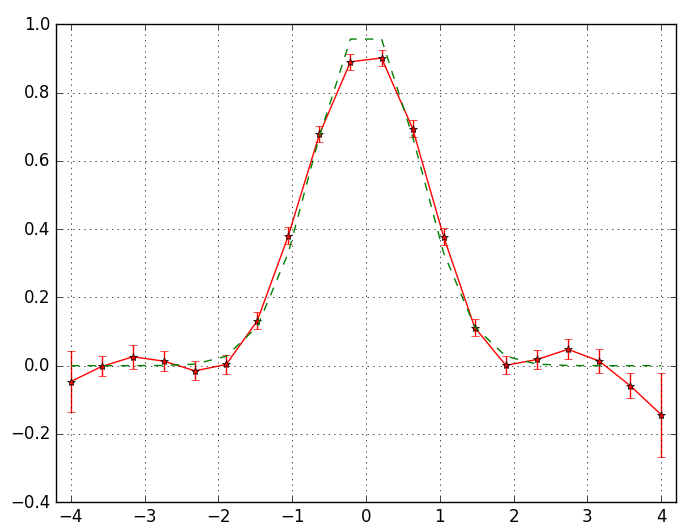
\includegraphics[width=1\linewidth]{no-negative1} \\а)
\end{minipage}
\hfill 
\begin{minipage}[h]{0.45\linewidth}
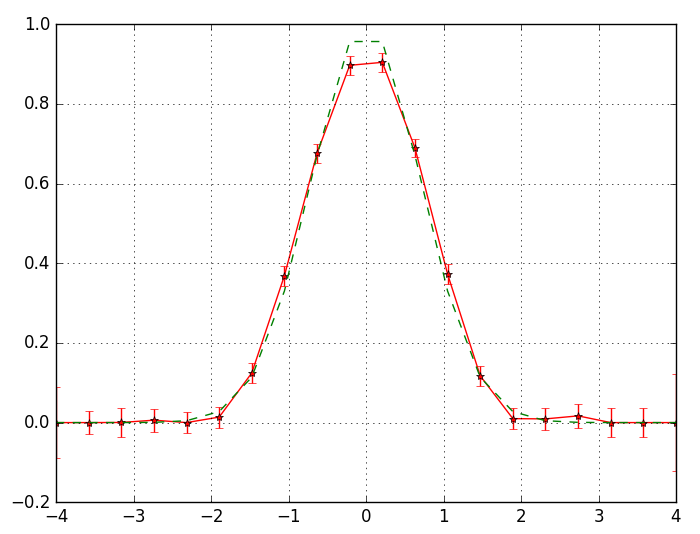
\includegraphics[width=1\linewidth]{no-negative2} \\б)
    \end{minipage}
    \caption{а) Результат регуляризации до добавления дополнительной информации. б) Результат оптимизации решения. Зеленая линия --- исходная функция, красная линия с точками --- результат регуляризации.}
\end{center}
\end{figure}
\end{comment}

\section{Исследование метода на примере данных эксперимента Troitsk nu-mass}
Рассмотрим работу метода в условиях обработки даных с реального физического эксперимента. Для проверки результата регуляризации были использованы данные измерения дифференциального сечения рассеяния электронов на изотопах водорода, полученные в эксперименте Troitsk nu-mass в 2015 году. Постановка задачи такая же: искомый спектр рассеянных элекронов сворачивается с известной разрешающей функцией спектрометра. В работе \cite{numass} приведены результаты обработки этих данных при помощи фитирования сложной функцией. Такой подход имеет два существенных недостатка:
\begin{enumerate}
    \item Функция, которой осуществляется фитирование подбирается ``на глаз'' и не имеет никакого физического обоснования. В частности таким образом невозможно исследовать особенности изучаемой функции, не заложенные в исходную модель.
    \item Имеют место сильные корреляции между параметрами фитирующей функции, которые сильно затрудняют фитирование, в некоторых случаях делая его невозможным.
\end{enumerate}
На Рис.\ref{pic:exp1} представлены экспериментальные данные - интегральный спектр рассеянных электронов. На Рис.\ref{pic:exp2} показаны результат регуляризации и результат фитирования. Регуляризация производилась с использованием базиса B-сплайнов с добавлением нулевых граничных условий. Как можно видеть, результат регуляризации хорошо согласуется с полученным ранее, однако можно еще улучшить результат, если добавить дополнительное условие неотрицательности функции, а также учесть влияние фона (площадка слева на экспериментальных данных Рис.\ref{pic:exp1}).
\newpage
\begin{figure}[htbp! ]
	\label{pic:6}
	\center{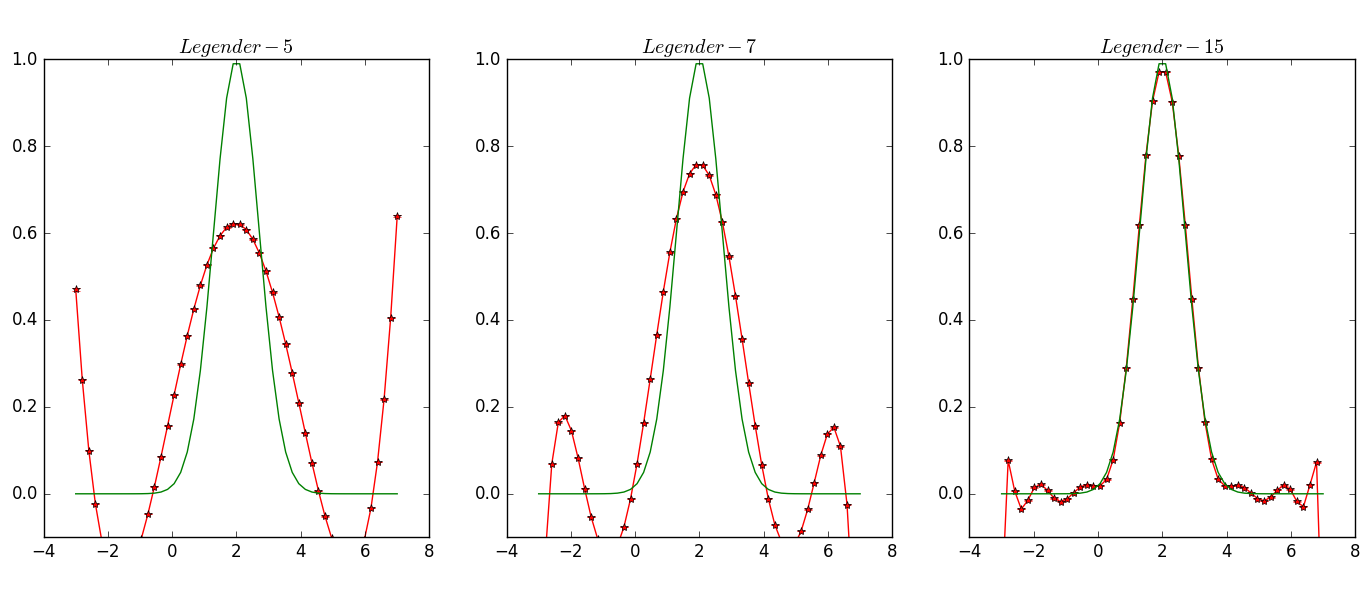
\includegraphics[width=1\linewidth]{pic6} }
	\caption{Восстановление функции Гаусса $e^{-(x-2)^2}$ с помощью 5, 7 и 15 полиномов Лежандра соответственно. Зеленая линия --- исходная функция, красная линия с точками --- результат восстановления.}
\end{figure}

\begin{figure}[htbp! ]
	\label{pic:7}
	\center{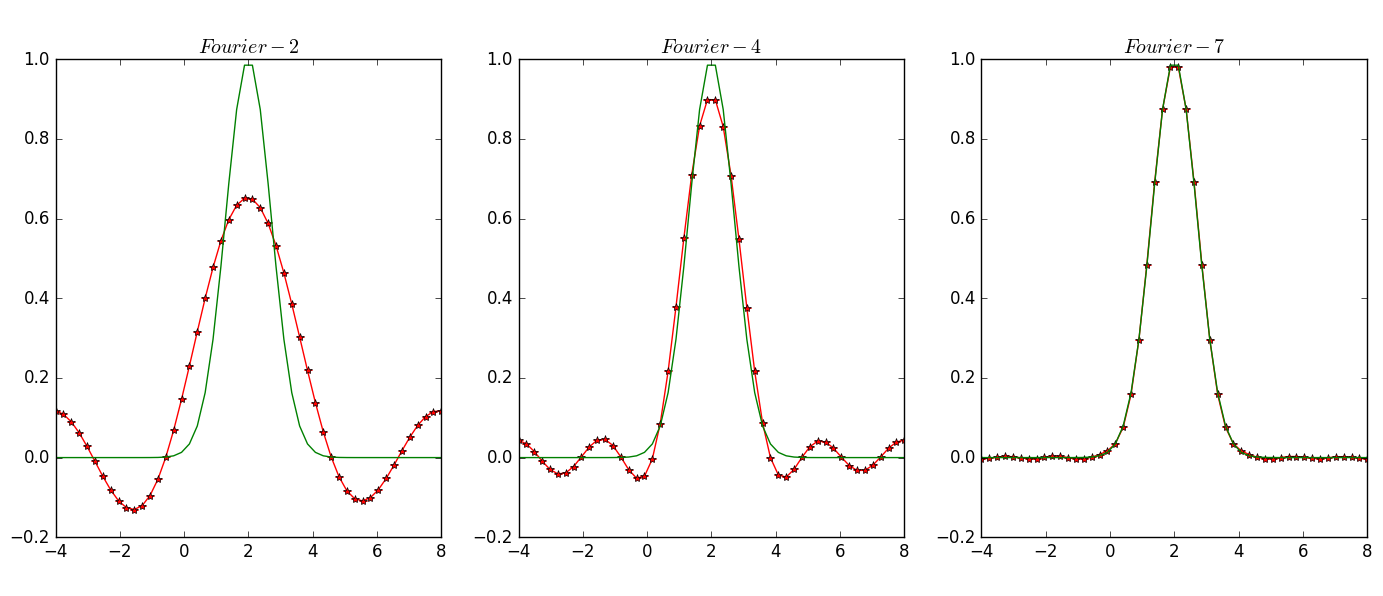
\includegraphics[width=1\linewidth]{pic7}}
	\caption{Восстановление функции Гаусса $e^{-(x-2)^2}$ с помощью 4, 8 и 14 компонент Фурье соответственно. Зеленая линия --- исходная функция, красная линия с точками --- результат восстановления.}
\end{figure}

\begin{figure}[htbp! ]
\begin{center}
\begin{minipage}[h]{0.3\linewidth}
	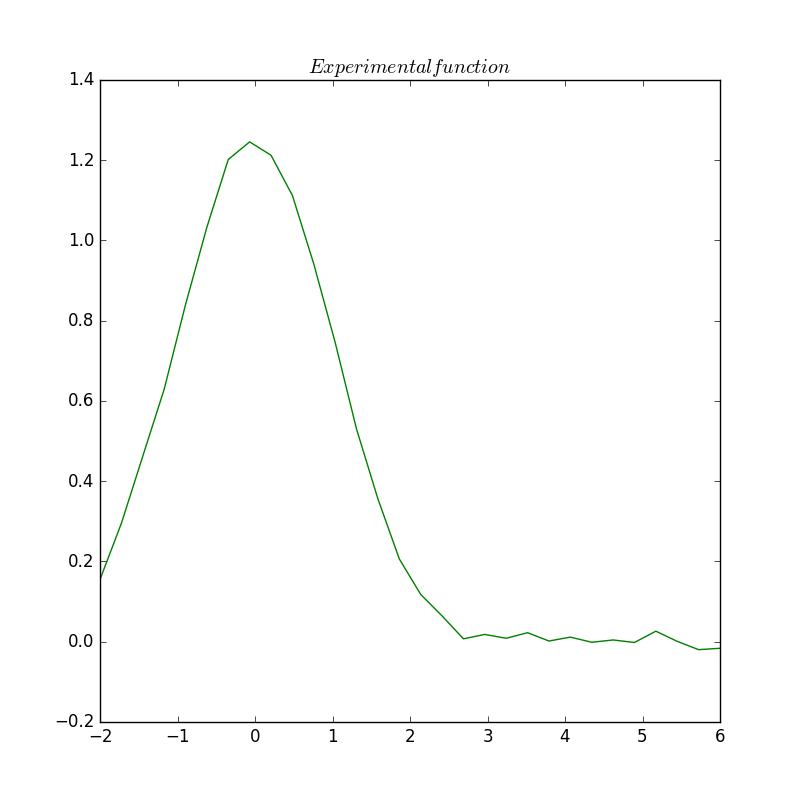
\includegraphics[width=1\linewidth]{func_10} \\а)
\end{minipage}
	\hfill
\begin{minipage}[h]{0.3\linewidth}
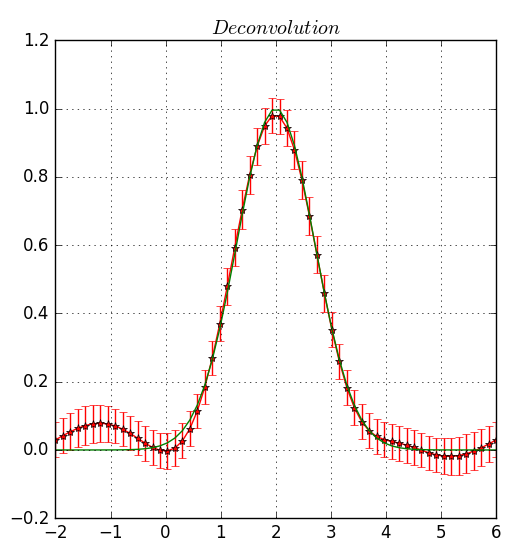
\includegraphics[width=1\linewidth]{pic10a} \\б)
\end{minipage}
\hfill
\begin{minipage}[h]{0.3\linewidth}
	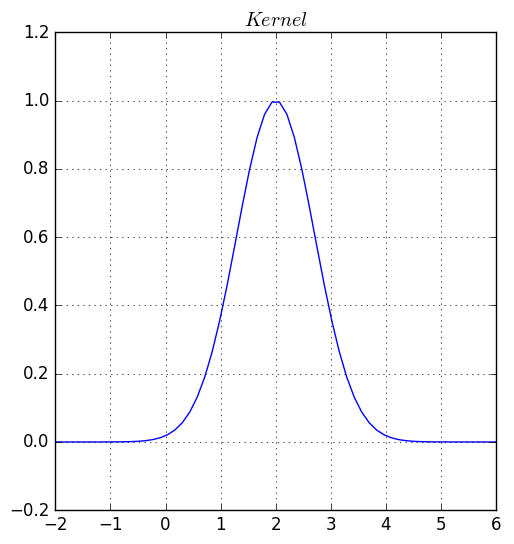
\includegraphics[width=1\linewidth]{pic10b} \\в)
\end{minipage}
	\caption{Случай неинтегрального ядра. а) Экспериментальные значения. б) Ядро $K=e^{-(x-2)^2}$. в) Результат восстановления с помощью базиса Фурье (20 компонент) со статистическими погрешностями 1\%, зеленая линия --- исходная функция, красная линия с точками --- результат регуляризации.}
\label{pic:gausskernel}
\end{center}
\end{figure}

\begin{figure}[htbp! ]
	\center{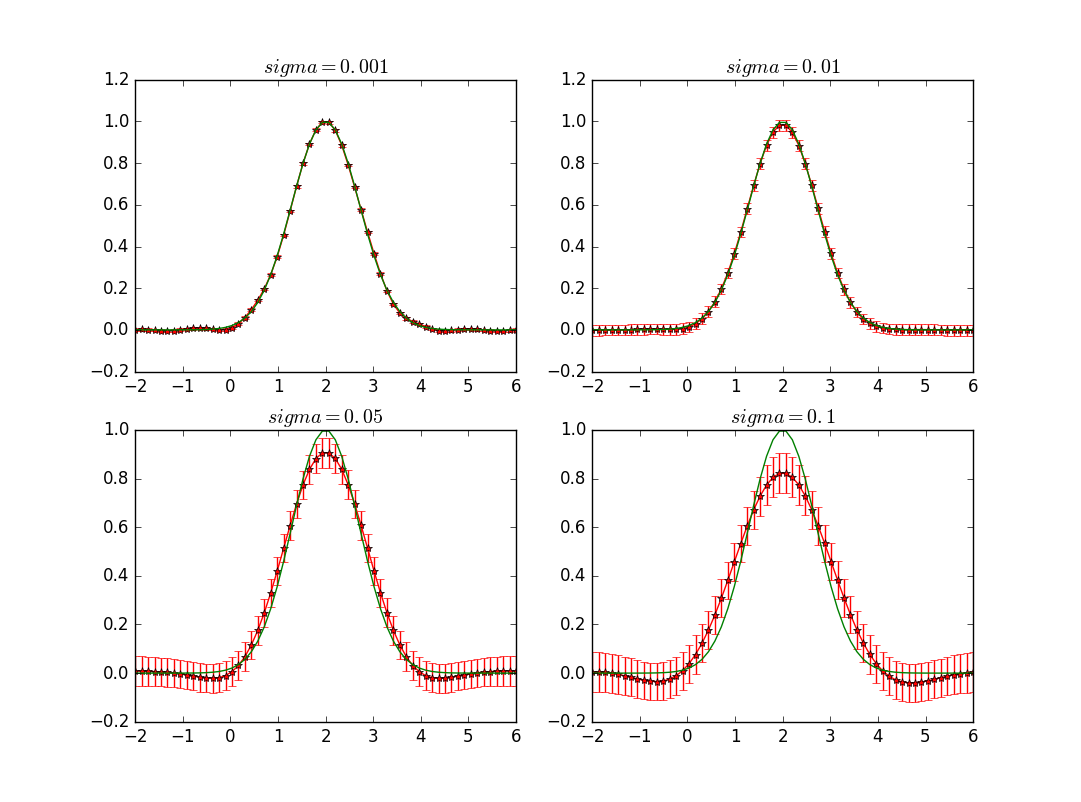
\includegraphics[scale=0.45]{pic12}}
	\caption{Восстановление гаусса с разными погрешностями при измерении: 0.001\%, 1\%, 5\% и 10\%. Зеленая линия --- исходная функция, красная линия с точками --- результат восстановления.}
	\label{pic:noize}
\end{figure}

\begin{figure}[htbp!]
\begin{center}
\begin{minipage}[h]{0.45\linewidth}
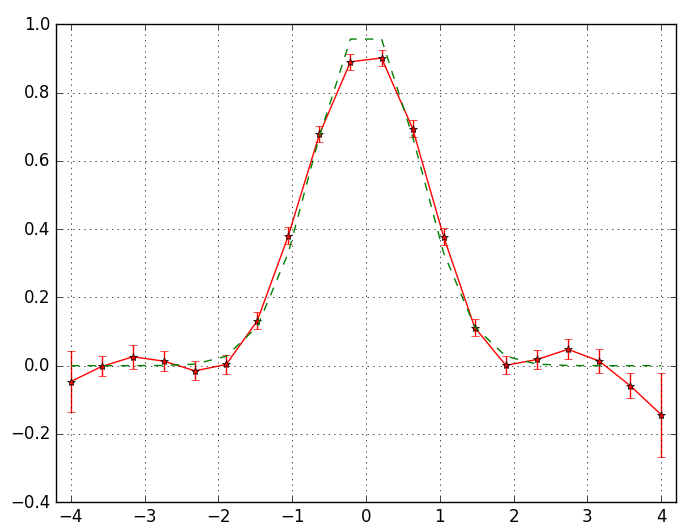
\includegraphics[width=1\linewidth]{no-negative1} \\а)
\end{minipage}
\hfill 
\begin{minipage}[h]{0.45\linewidth}
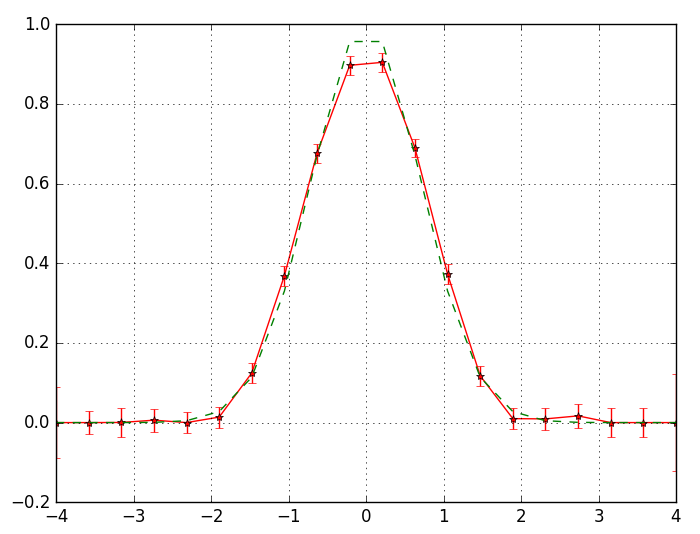
\includegraphics[width=1\linewidth]{no-negative2} \\б)
\end{minipage}
\caption{а) Результат регуляризации до добавления дополнительной информации. б) Результат оптимизации решения. Зеленая линия --- исходная функция, красная линия с точками --- результат регуляризации.}
\label{pic:aprioriopt}
\end{center}
\end{figure}

\begin{figure}[htbp! ]
	\label{pic:exp1}
	\center{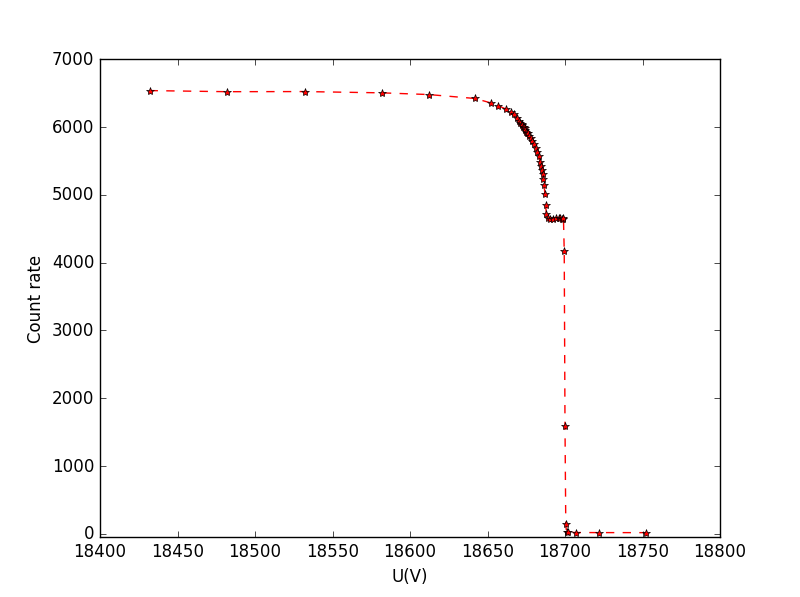
\includegraphics[width=1\linewidth]{exper_data}}
	\caption{Экспериментальные данные --- спектр рассеянных электронов при энергии пушки 18700 eV.}
\end{figure}

\begin{figure}[htbp! ]
	\label{pic:exp3}
	\center{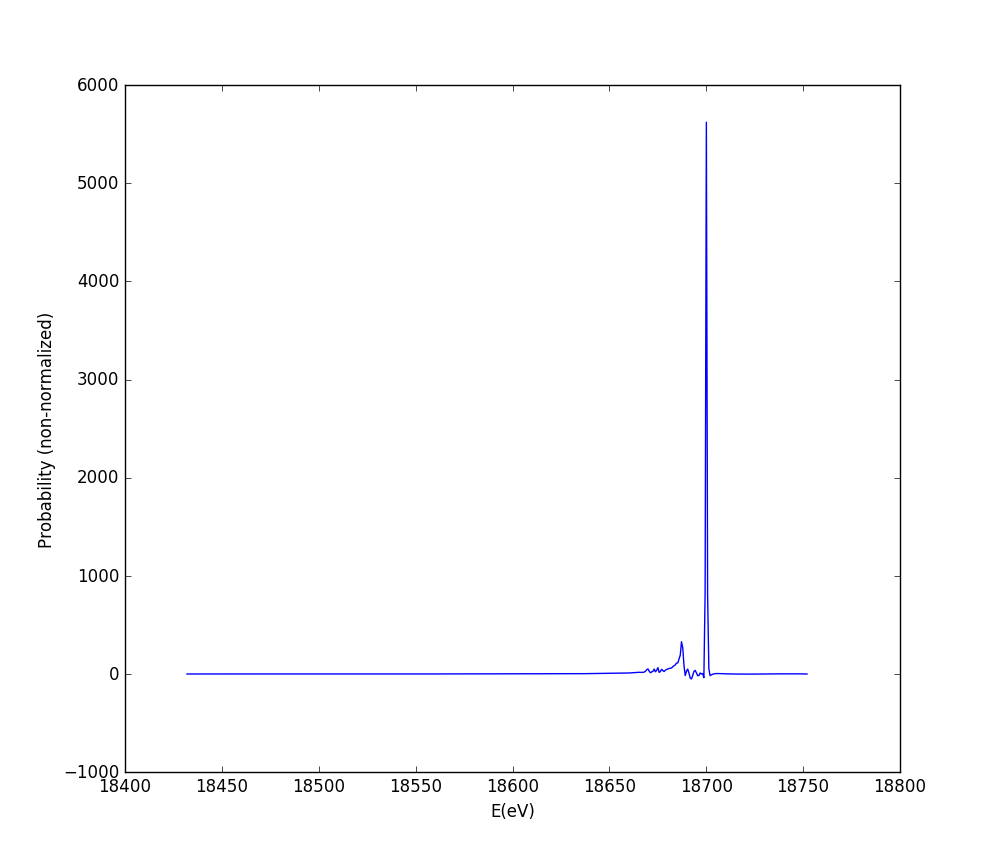
\includegraphics[width=0.75\linewidth]{exp_full}}
	\caption{Результат обработки данных эксперимента Троицк ню-масс.}
\end{figure}

\begin{figure}[htbp! ]
	\label{pic:exp2}
	\center{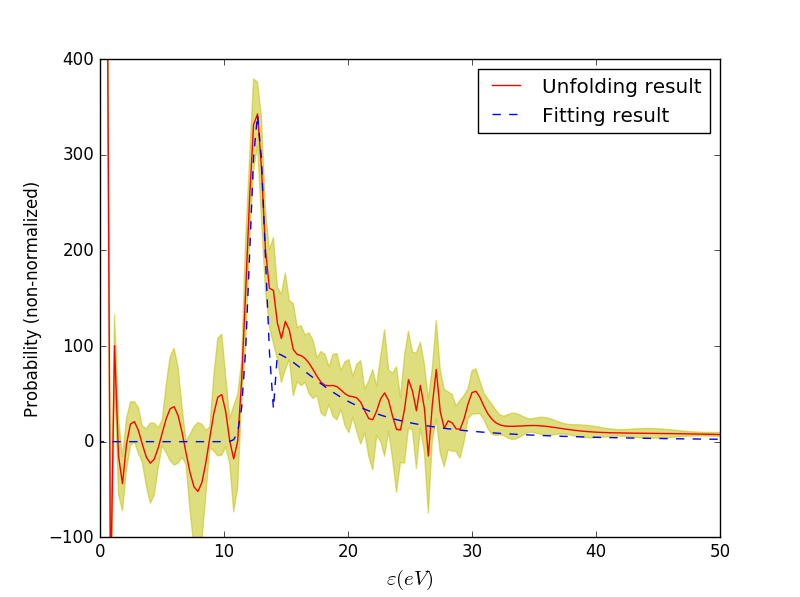
\includegraphics[width=0.75\linewidth]{experim}}
	\caption{Результат обработки данных эксперимента Троицк ню-масс (красная линия) и результат фитирования (пунктирная линия), область одинарного рассеяния.}
\end{figure}
\newpage
\likechapter{Заключение}

Был реализован и исследован метод статистической регуляризации Турчина, с использованием трех различных методов алгебраизации. В результате работы сделаны следующие выводы: 
\begin{itemize}
\item Существенное преимущество метода регуляризации Турчина заключаются в существовании конкретного аналитического способа нахождения параметра регуляризации и погрешностей найденного решения.
 
\item Анализ восстановления модельных задач показал зависимость результата регуляризации от способа алгебраизации, а также параметров выбранного базиса (количество базисных функций, количество узлов). Однако для каждого базиса существуют соответствующие оптимальные параметры, следовательно для каждой задачи возможно подобрать наиболее подходящий базис.

\item Метод статистической регуляризации Турчина основан на Байесовом подходе, что дает возможность использования дополнительной априорной информации. Было реализовано добавление дополнительной априорной информации о неотрицательности функции путем оптимизации уже найденного решения, а также добавление граничных условий для базиса B-сплайнов. Использование апостериорной вероятности предполагает возможную реализацию всей доступной априорной информации о свойствах искомой функции.

\item Данный метод регуляризации был применен для обработки данных калибровочных измерений с эксперимента ``Троицк ню-масс''. Результаты регуляризации хорошо согласуются с результатами, полученными ранее при использовании стандартных методов обработки, что подтверждает работоспособность метода в условиях реального физического эксперимента.
 \end{itemize}
 
\hfill \break
\hfill \break

Автор данной работы выражает глубокую признательность своему научному руководителю Нозику Александру Аркадьевичу за постановку интересной задачи, активное руководство, а также проявленное терпение и внимание. 

Я также глубоко благодарна Михаилу Зеленому и Алексею Худякову за неоценимую помощь, многочисленные советы, обсуждения и терпеливые объяснения.

Мне приятно также поблагодарить Нозика Валерия Зиновьевича за полезные обсуждения полученных результатов и помощь в подготовке данной дипломной работы.
 
 

\newpage
\renewcommand {\appendixtocname} {ПРИЛОЖЕНИЯ}
\appendixtocon
\begin{appendices}
    \chapter{Вывод метода}
\label{sec:metod}

Докажем формулу (\ref{eq:apriori}). Для поиска условного экстремума используем метод Лагранжа. Функция Лагранжа:
\begin{equation}
L(\vec{\varphi}, \lambda, \mu) = \ln{P(\vec{\varphi})} P(\vec{\varphi}) + \lambda (\vec{\varphi},\Omega\vec{\varphi}) P(\vec{\varphi}) + \mu P(\vec{\varphi})
\end{equation}
Подставляем её в уравнение Эйлера-Лагранжа:
\begin{equation}
\frac{\partial L}{\partial \varphi} = P'(\vec{\varphi})(1 + \ln{P(\vec{\varphi})}  + \lambda (\vec{\varphi},\Omega\vec{\varphi}) + \mu ) = 0
\end{equation}
Получаем два варианта. Решение уравнения $P'(\vec{\varphi}) = 0$ не очень интересно, поскольку возвращает нас к равновероятным $\vec{\varphi}$ и не регуляризованному решению.
Интересное решение:
\begin{equation}
P(\vec{\varphi}) = \exp(-1 + \mu + \lambda (\vec{\varphi},\Omega\vec{\varphi}))
\label{eq:eqlagr}
\end{equation}
Обычно следует подставить эту функцию в условия и получить значения параметров $\lambda$ и $\mu$. Но мы пойдем другим путем. Сделаем замену переменных: $\lambda = -\frac{\alpha}{2}$, $ C=\exp(-1 + \mu)$ и подставим в (\ref{eq:eqlagr}):
\begin{equation}
P(\vec{\varphi}) = C\exp(-\frac{\alpha}{2} (\vec{\varphi},\Omega\vec{\varphi}))
\end{equation}
Сравним полученную формулу с многомерным гаусоввым распределением:
\begin{equation}
f_X(\vec{x}) = \frac{1}{(2\pi)^{n/2}|\Sigma|^{1/2}} \exp(-\frac{1}{2}(\vec{x} - \vec{\mu})^T\Sigma^{-1}(\vec{x} - \vec{\mu}))
\end{equation}
Отсюда можно сделать вывод: $C =  \frac{1}{(2\pi)^{N/2}|\Sigma|^{1/2}}$, $\Sigma^{-1} = \alpha\Omega$, $|\Sigma| = \frac{1}{|\Sigma^{-1}|} = \frac{1}{\alpha^{Rg(\Omega)}|\Omega|}$, а:
\begin{equation}
P_{\alpha}(\vec{\varphi})  = \frac{\alpha^{Rg(\Omega)/2}\det\Omega^{1/2}}{(2\pi)^{N/2}} \exp(-\frac{1}{2} (\vec{\varphi},\alpha\Omega\vec{\varphi}))
\end{equation}
    \chapter{Вывод формул в гауссовом случае} \label{sec:gauss}

Покажем что для определения наиболее вероятного $\alpha$ следует искать максимум функции (\ref{eq:alphamax}).По теореме Байеса:

\begin{equation}
	P(\alpha|\vec{f}) \sim P(\alpha)P(\vec{f}|\alpha),
\end{equation}
где
\begin{equation}
	\label{eq:prob_f_alpha}
	P(\vec{f}|\alpha) = \int d\vec{\varphi} P(\vec{f}|\vec{\varphi})P(\vec{\varphi}|\alpha)
\end{equation}

Введем дополнительные обзначения: $b^T = \vec{f}^T\Sigma^{-1}K$, $B = K^T\Sigma^{-1}K$.
Тогда: $\vec{f}^T\Sigma^{-1}\vec{f} = \vec{f}\Sigma^{-1}K^{T}K^{-1T}\Sigma^{T}\Sigma^{-1T} KK^{-1}\vec{f} = b^{T}B^{-1}b$, a:

\begin{equation}
	\label{eq:aposteoriphi}
	P(\vec{f}|\vec{\varphi})P(\vec{\varphi}|\alpha) = \frac{\alpha^{Rg(\Omega)/2}\det\Omega^{1/2}}{(2\pi)^{(N+M)/2}|\Sigma|^{1/2}}\exp(-\frac{1}{2}b^{T}B^{-1}b) \exp(-\frac{1}{2} (\vec{\varphi},(B+\alpha\Omega)\vec{\varphi}) + b\vec{\varphi})
\end{equation}

Посчитаем интеграл (\ref{eq:prob_f_alpha}), воспользовавшись его сходством с многомерным нормальным распределением:

\begin{equation}
	P(\vec{f}|\alpha) = \frac{\alpha^{Rg(\Omega)/2}|\Omega^{1/2}|}{(2\pi)^{(M)/2}|\Sigma|^{1/2}}\exp(-\frac{1}{2}b^{T}B^{-1}b) \sqrt{|(B+\alpha\Omega)^{-1}|}\exp(\frac{1}{2}b^{T}(B+\alpha\Omega)^{-1}b)
\end{equation}

По теореме Байеса мы можем определить $P(\alpha|\vec{f})$ ($C$ не зависит от $\alpha$):

\begin{equation}
	\label{eq:alphaaposter}
	P(\alpha|\vec{f}) = C \alpha^{\frac{Rg(\Omega)}{2}}\sqrt{|(B+\alpha\Omega)^{-1}|}\exp(-\frac{1}{2}b^{T}B^{-1}b)\exp(\frac{1}{2}b^{T}(B+\alpha\Omega)^{-1}b)
\end{equation}

Предпологая, что $P(\alpha|\vec{f})$ должно иметь узкий пик для некоторого $\alpha:*$, мы будем искать экстремум логарифма $P(\alpha|\vec{f})$:

\begin{equation}
	\ln{P(\alpha|\vec{f})} = \ln{C} + \frac{Rg(\Omega)}{2}\ln{\alpha} - \frac{1}{2}\ln{|B+\alpha\Omega|}  + \frac{1}{2}b^{T}(B+\alpha\Omega)^{-1}b
\end{equation}
    \chapter{Алгебраизация}
\label{algebra}

Для алгебраизации уравнения , мы разложим функцию $\varphi(x)$, по некоторой системе функций $\{T_n\}$:
\begin{equation}
\varphi(x) = \sum \limits_n \varphi_n T_n(x).
\end{equation}
Таким образом компонентами вектора $\vec{\varphi}$ являются коэффициенты этого разложения. Тогда элементы матрицы $K$, вычисляются как:
\begin{equation}
K_{mn} = \int\limits_a^b K(x,y_m)T_n(x)dx,
\end{equation}
а элементы матрицы $\Omega$ по формуле:
\begin{equation}
\Omega_{ij} = \int\limits_a^b \left(\frac{dT_i(x)}{dx}\right)\left(\frac{dT_j(x)}{dx}\right)dx. 
\end{equation}
Для пересчета ошибок следует использовать формулу дисперсии линейной комбинации случайных величин:
\begin{equation}
D[\varphi(x)] = D[\sum \limits_n \varphi_n T_n(x)] = \sum\limits_{i,j} \varphi_i\varphi_j cov(T_i(x), T_j(x)).
\end{equation}

    \chapter{Базис полиномов Лежандра}\label{sec:legendre}

Базис представляет собой набор n первых полиномов Лежандра:
$$P_n(z)=\frac{1}{2^n n!}\frac{d^n}{dz^n}(z^2-1)^n$$
Такая система ортогональна на отрезке [-1,1], но этот отрезок может быть переопределен заменой переменной в полиномах.
\begin{figure}[h!]
	\begin{minipage}[h]{0.49\linewidth}
		\center{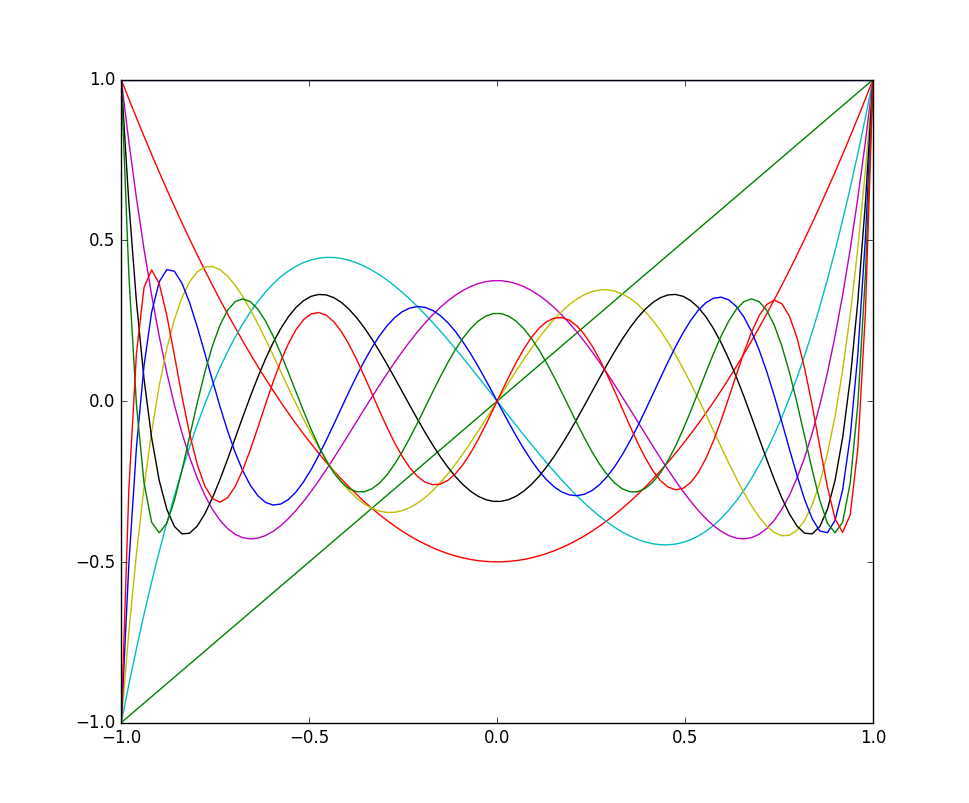
\includegraphics[scale=0.25]{figure_1}}
		\center{\caption{Базисные функции}}
	\end{minipage}
\hfill
	\begin{minipage}[h]{0.49\linewidth}
		\center{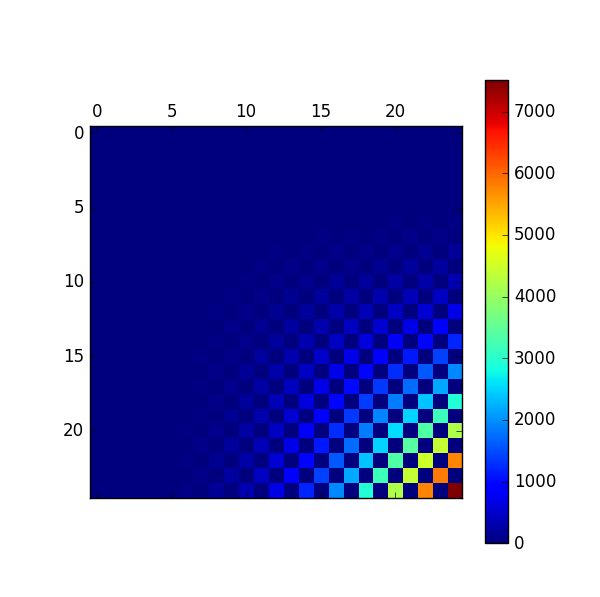
\includegraphics[scale=0.4]{figure_2}}
		\caption{Матрица $\Omega$}
	\end{minipage}
\label{ris:image1}
\end{figure}
Производится разложение функции в ряд вида
$$f(\mu)=a_0 P_0 (\mu) + a_1 P_1 (\mu) + ... +  a_n P_n (\mu),$$
$-1 < \mu <1 .$
Коэффициенты разлодения определяются как:
$$a_m = \frac{1}{2}(2m+1)\int\limits_{-1}^{1}f(\mu)P_m (\mu)d\mu .$$
Такая система ортогональна на отрезке [-1,1], но этот отрезок может быть переопределен заменой переменной в полиномах.

\section{Базис Фурье}\label{sec:fourier}

В качестве Фурье базиса используется тригонометрический ряд Фурье \{$\sin nx, \cos nx$\}.
Разложение функции по базису производится по формулам:
$$f(x)=\frac{a_0}{2} + \sum^{\infty}_{n=1} (a_n \cos nx + b_n \sin nx)$$
где
$$a_0= \frac{1}{\pi}\int\limits_{-\pi}^{\pi}f(x)dx,$$
$$a_n= \frac{1}{\pi}\int\limits_{-\pi}^{\pi}f(x)\cos(nx)dx,$$
$$b_n= \frac{1}{\pi}\int\limits_{-\pi}^{\pi}f(x)\sin(nx)dx.$$

\section{B-сплайны}\label{sec:spline}

B-сплайны (базисные сплайны) --- базисные функции, использующиеся для апроксимации ломаных. Кривая, построенная на основе B-сплайн-базиса, описывается следующим образом:
$$\vec{p}(t)=\sum^{n}_{i=0} \vec{P_i}N_{ik} (t),$$
где $\vec{p}(t)$ --- радиус-вектор точек на кривой, $\vec{P_i}$ --- вершины аппроксимируемой ломаной (всего вершин n+1), а $N_{ik} (t)$ --- весовая функция ш-й нормальзованноый B-сплайн базисной кривой порядка k (т.е. степени k-1), задаваемая рекурентными соотношениями:
\begin{equation*}
N_{i1} = 
 \begin{cases}
   1, &\text{если $x_i \leq t \leq x_{i-1},$}\\
   0, &\text{если $t \notin (x_i, x_{i-1})$}
 \end{cases}
\end{equation*}
$$ N_{ik} (t) = \frac{(t-x_i)N_{i,k-1}(t)}{x_{i+k-1} - x_i} - \frac{(x_{i+k}-t)N_{i+1,k-1}(t)}{x_{i+k} - x_{i+1}} .$$
Здесь $x_i$ --- элементы узлового вектора, а t – параметр, изменяю­щийся в диапазоне от 0 до $t_{max}=(n – k+2)$.
B-сплайн-кривая является полиномом степени (k–1) на каждом интервале $(x_i, x_{i+1})$, и все ее производные до (k–2)-го порядка включительно непрерывны вдоль всей кривой. То есть эта кривая представляет собой сплайн-функцию порядка k (степени k–1).

    \chapter{Некоторые функции}

\section{Crystal Ball}\label{sec:crystalball}

Функция Crystal Ball --- функция плотности вероятности, часто используемая для описания потерь энергии в физике высоких энергий.
$$f(x;\alpha,n,\bar x,\sigma) = N \cdot \begin{cases} \exp(- \frac{(x - \bar x)^2}{2 \sigma^2}), & \mbox{for }\frac{x - \bar x}{\sigma} > -\alpha \\
 A \cdot (B - \frac{x - \bar x}{\sigma})^{-n}, & \mbox{for }\frac{x - \bar x}{\sigma} \leq -\alpha \end{cases}$$
где
$$A = \left(\frac{n}{\left| \alpha \right|}\right)^n \cdot \exp\left(- \frac {\left| \alpha \right|^2}{2}\right),$$
$$B = \frac{n}{\left| \alpha \right|}  - \left| \alpha \right|,$$
$$N = \frac{1}{\sigma (C + D)},$$
$$C = \frac{n}{\left| \alpha \right|} \cdot \frac{1}{n-1} \cdot \exp\left(- \frac {\left| \alpha \right|^2}{2}\right),$$
$$D = \sqrt{\frac{\pi}{2}} \left(1 + \operatorname{erf}\left(\frac{\left| \alpha \right|}{\sqrt 2}\right)\right).$$
В работе использовалась функция Crystal Ball с параметрами $\alpha=1, n=2, x_0=0, \sigma=1$.

\section{Сигмоида}\label{sec:sigmoida}

Сигмоида --- гладкая монотонная нелинейная функция, имеющая форму буквы "S". В нашем случае использовалась сигмоида вида:
$$\sigma(x) = \frac{1}{1+e^{-x}}.$$

\end{appendices}


\newpage
\addcontentsline{toc}{chapter}{Литература}
\bibliography{lit}
\end{document}
